\title[ASD - Analisi di algoritmi]{\textbf{Algoritmi e Strutture Dati}\\[18pt]Analisi di algoritmi\\Ricorrenze, metodo di sostituzione}

%-------------------------------------------------------------------------
\FrameTitle{}

%%%%%%%%%%%%%%%%%%%%%%%%%%%%%%%%%%%%%%%%%%%%%%%%%%%%%%%%%%%%%%%%%%%%%%%%%%
\subsection{Metodo della sostituzione}

%\subsubsection{Introduzione}

\begin{frame}{Metodo della sostituzione}

\vspace{-6pt}
\begin{myboxtitle}[Metodi per risolvere ricorrenze]
\BI
\item Metodo dell'albero di ricorsione, o per livelli
\item \alert{Metodo di sostituzione, o per tentativi}
\item Metodo dell'esperto, o delle ricorrenze comuni
\EI
\end{myboxtitle}


\begin{myboxtitle}[Metodo di sostituzione]
\`E un metodo in cui si cerca di “\alert{indovinare}”  (guess) una soluzione, in base alla propria esperienza,
e si dimostra che questa soluzione è corretta tramite \alert{induzione}.
\end{myboxtitle}

\end{frame}

%\subsubsection{Primo esempio}

\begin{frame}[shrink=5]{Cerchiamo di indovinare}

\vspace{-6pt}
\begin{mybox}
\begin{columns}[c]
\begin{column}{0.46\textwidth}
\[
T(n) = \begin{cases}
      T( \lfloor n/2 \rfloor )  + n & n > 1 \\
     1 & n \leq 1
  \end{cases}
\]
\end{column}
\begin{column}{0.51\textwidth}
\end{column}
\end{columns}
\end{mybox}


\begin{overprint}
\onslide<2|handout:0>
\begin{figure}
	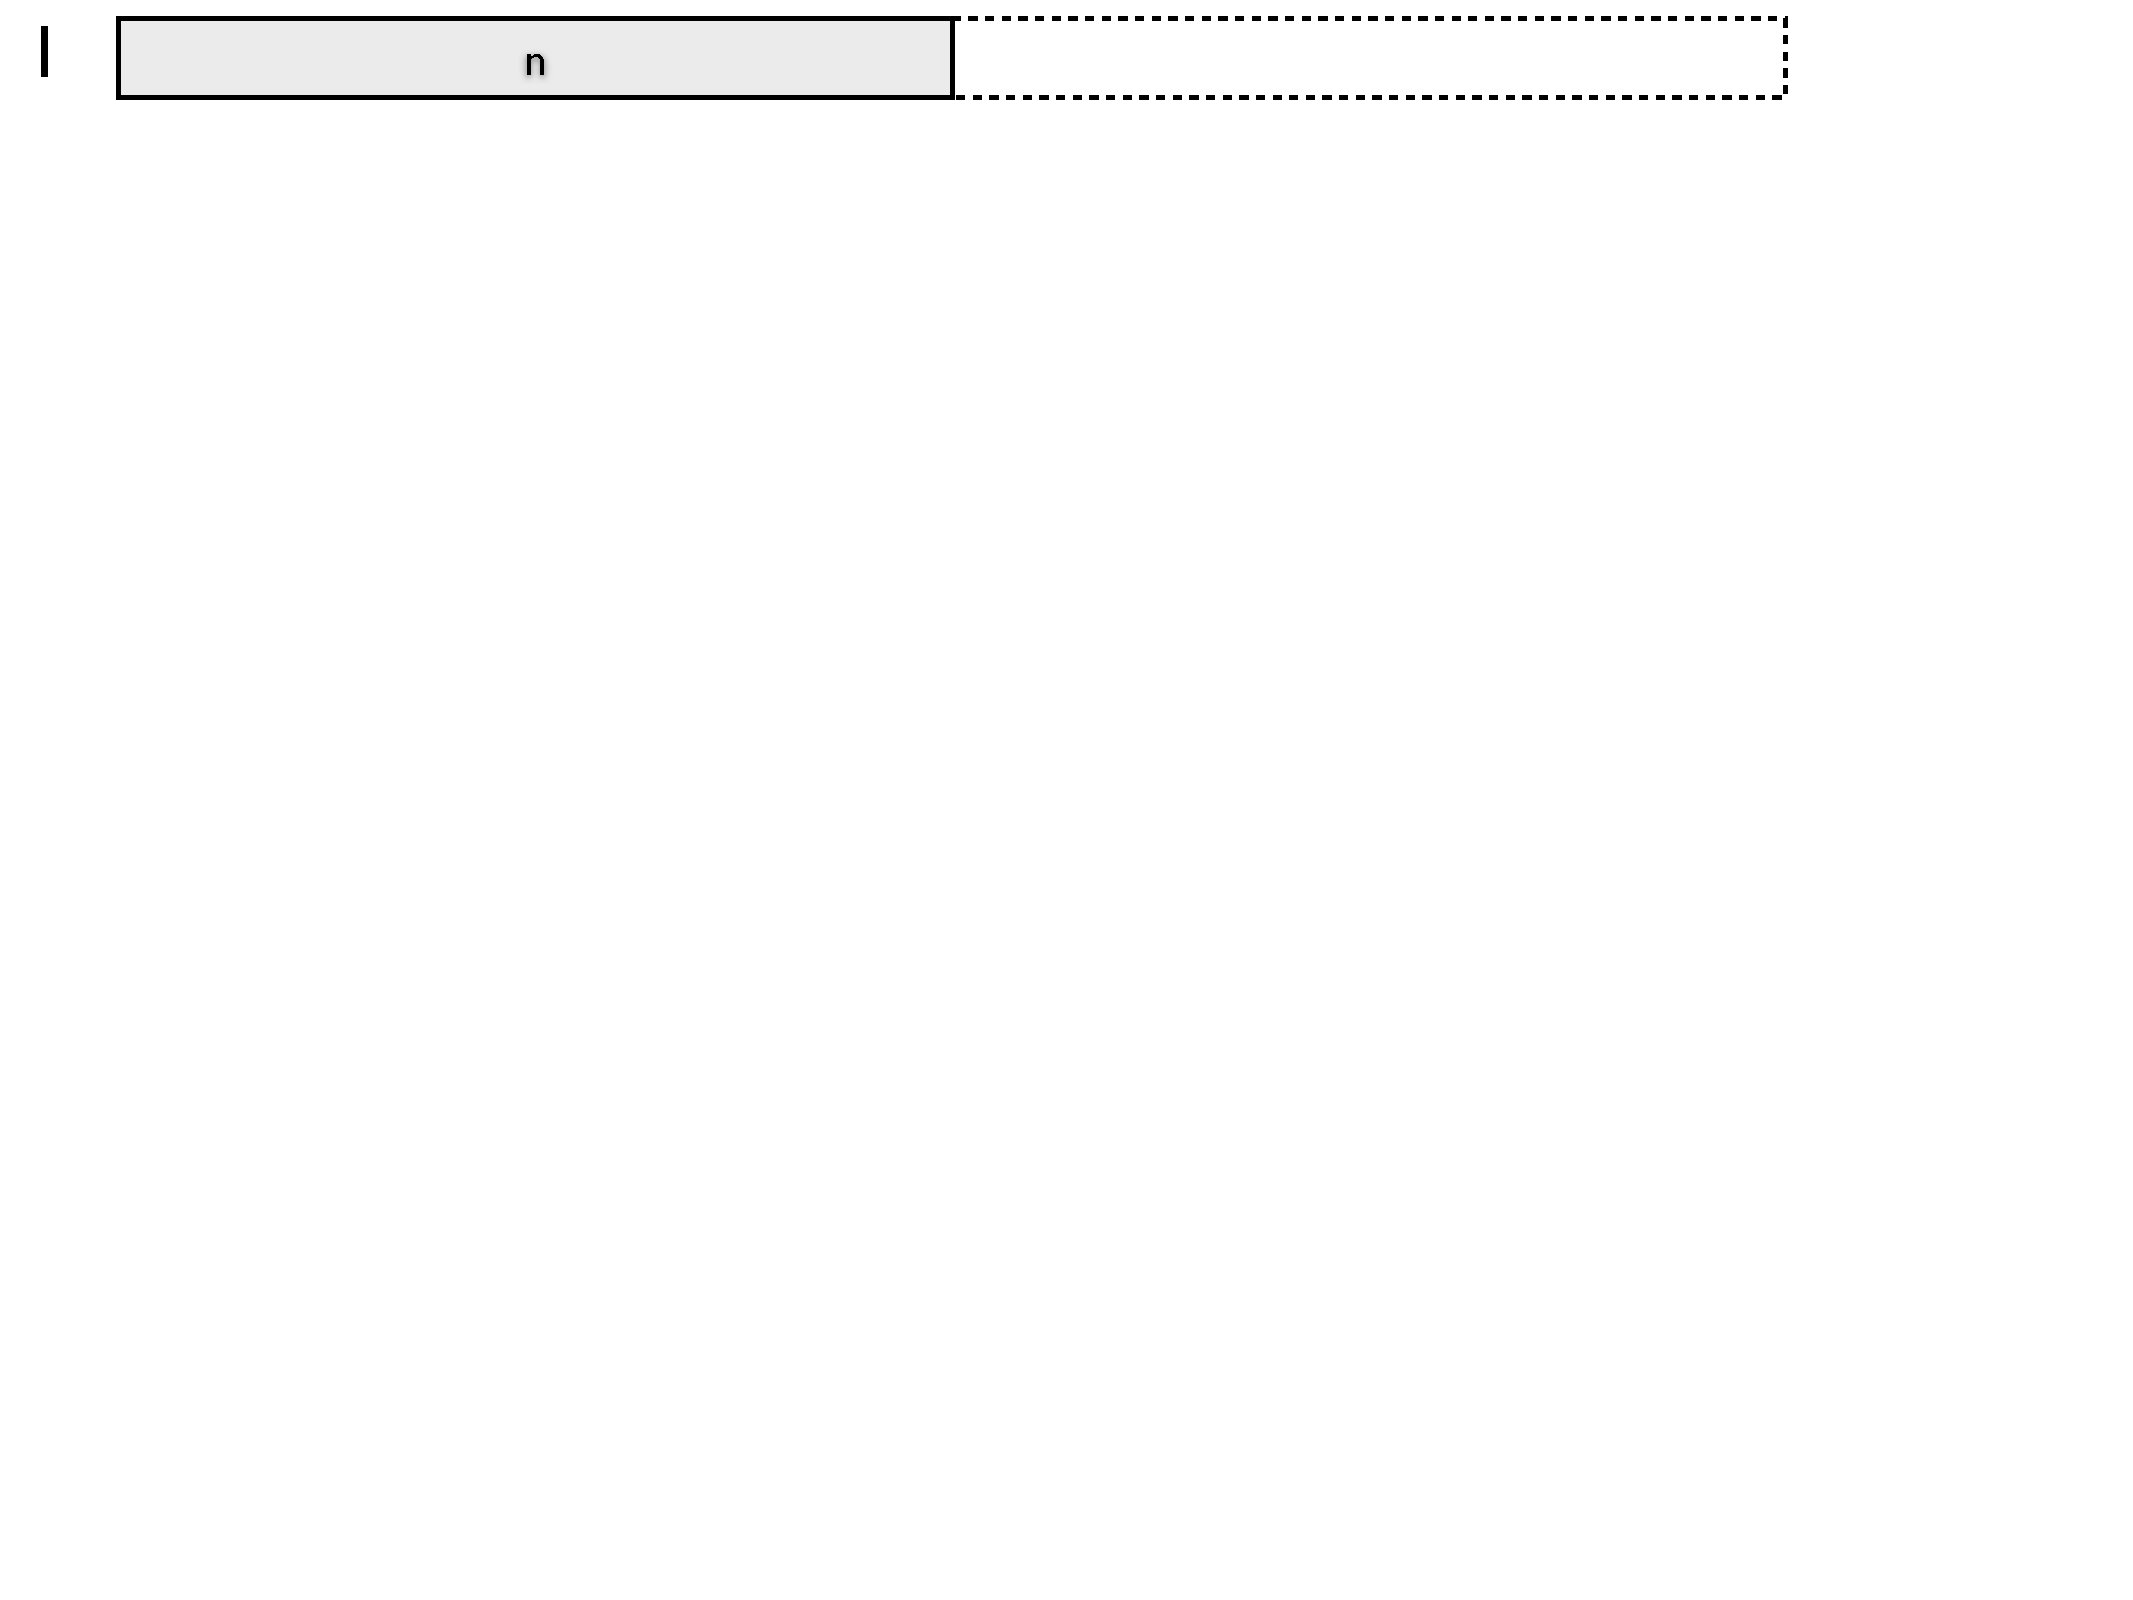
\includegraphics[width=0.8\textwidth,page=1,trim=0 20 10 0]{achille.pdf}
\end{figure}
\onslide<3|handout:0>
\begin{figure}
	\includegraphics[width=0.8\textwidth,page=2,trim=0 20 10 0]{achille.pdf}
\end{figure}
\onslide<4|handout:0>
\begin{figure}
	\includegraphics[width=0.8\textwidth,page=3,trim=0 20 10 0]{achille.pdf}
\end{figure}
\onslide<5|handout:0>
\begin{figure}
	\includegraphics[width=0.8\textwidth,page=4,trim=0 20 10 0]{achille.pdf}
\end{figure}
\onslide<6|handout:0>
\begin{figure}
	\includegraphics[width=0.8\textwidth,page=5,trim=0 20 10 0]{achille.pdf}
\end{figure}
\onslide<7|handout:0>
\begin{figure}
	\includegraphics[width=0.8\textwidth,page=6,trim=0 20 10 0]{achille.pdf}
\end{figure}
\onslide<8|handout:1>
\begin{figure}
	\includegraphics[width=0.8\textwidth,page=7,trim=0 20 10 0]{achille.pdf}
\end{figure}
\onslide<9|handout:2>
\[
  T(n) =    {n \cdot \sum_{i=0}^{ \log n } (1/2)^i}
       ~\textcolor{red}{\leq}~ {n \cdot \sum_{i=0}^{\infty} (1/2)^i}
       = {n \cdot \frac{1}{1-\frac{1}{2}} = 2n}
\]

\begin{myboxtitle}[Serie geometrica decrescente infinita]
\[
 \forall x, |x|<1: \sum_{i=0}^{\infty} x^i = \frac{1}{1-x}
\]
\end{myboxtitle}
\end{overprint}
\end{frame}





\begin{frame}[shrink=5]{Limite superiore}
	
\vspace{-6pt}
\begin{mybox}
\begin{columns}[c]
\begin{column}{0.46\textwidth}
\[
T(n) = \begin{cases}
      T( \lfloor n/2 \rfloor )  + n & n > 1 \\
     1 & n \leq 1
  \end{cases}
\]
\end{column}
\begin{column}{0.51\textwidth}
\begingroup\small
\alert{Tentativo: $T(n) = O(n)$}\\[2pt]
$\exists c > 0, \exists m \geq 0:T(n) \leq cn, \forall n \geq m$
\endgroup
\end{column}
\end{columns}
\end{mybox}


\begin{overprint}
\onslide<1|handout:1>
\BI
\item {\bf Caso base}: Dimostriamo la disequazione per $T(1)$
	\begin{flalign*}
       T(1) &= 1 \stackrel{?}{\leq} 1 \cdot c \Leftrightarrow {\forall c \geq 1} &&
    \end{flalign*}
\EI
\onslide<2|handout:2>
\BIL
\item \textbf{Ipotesi induttiva}: $\alert{\forall k < n: T(k) \leq c k}$.
\item \textbf{Passo di induzione}: Dimostriamo la disequazione per $T(n)$\\[-6pt]
\begin{flalign*}
  T(n) &=    {T(\lfloor n/2 \rfloor) + n} \\
       &\leq {c \lfloor n/2 \rfloor + n} && \text{Sostituzione} \\
       &\leq {c n/2 + n} && \text{Intero inferiore} \\
       &=    {(c/2 + 1)n} && \text{Passo algebrico} \\
       &\stackrel{?}{\leq} {cn} && \text{Obiettivo} \\
       &\Leftrightarrow  {c/2+1 \leq  c} \Leftrightarrow  {c \geq 2} && \text{Risultato finale} 
\end{flalign*}
\EIL

\onslide<3|handout:3>
\BIL
	\item Abbiamo provato che $T(n) \leq cn$
	\BI
		\item \makebox[3.5cm][l]{Nel caso base:} $c \geq 1$
		\item \makebox[3.5cm][l]{Nel passo induttivo:} $c \geq 2$
		\item Un valore $c$ che rispetta entrambe le disequazioni è $c=2$
	\EI
	\item Questo vale per $n=1$, e per tutti i valori di $n$ seguenti
	\BI
		\item Quindi $m=1$
	\EI
\EIL

\begin{mybox}
	Abbiamo quindi provato che $T(n)=O(n)$
\end{mybox}

\end{overprint}


\end{frame}


\begin{frame}[shrink=5]{Limite inferiore}


\vspace{-6pt}{}
\begin{mybox}
\begin{columns}[c]
\begin{column}{0.46\textwidth}
\[
T(n) = \begin{cases}
      T( \lfloor n/2 \rfloor )  + n & n > 1 \\
     1 & n \leq 1
  \end{cases}
\]
\end{column}
\begin{column}{0.51\textwidth}
\alert{Tentativo: $T(n) = \Omega(n)$}\\[2pt]
$\exists d > 0, \exists m \geq 0:T(n) \geq dn, \forall n \geq m$
\end{column}
\end{columns}
\end{mybox}



\begin{overprint}
\onslide<1|handout:1>
\BI
\item {\bf Caso base}: Dimostriamo la disequazione per $T(1)$
	\begin{flalign*}
     T(1) &= 1 \stackrel{?}{\geq} 1 \cdot d \Leftrightarrow {\forall d \leq 1} &&
  \end{flalign*}
\EI
\onslide<2|handout:2>
\BIL
\item \textbf{Ipotesi induttiva}: $\alert{\forall k < n: T(k) \geq d k}$.
\item \textbf{Passo di induzione}: Dimostriamo la disequazione per $T(n)$\\[-6pt]
\begin{flalign*}
  T(n) &=    {T(\lfloor n/2 \rfloor) + n} \\
       &\geq {d \lfloor n/2 \rfloor + n} && \text{Sostituzione} \\
       &\geq {dn/2-1 + n} && \text{Intero inferiore} \\
       &=    {\left( \frac{d}{2} - \frac{1}{n} + 1 \right) n} \stackrel{?}{\geq} {dn}  && \text{Passo algebrico}  \\
%       && \text{Obiettivo} \\
       &\Leftrightarrow  {\frac{d}{2}-\frac{1}{n} + 1 \geq  d} \Leftrightarrow  { d \leq 2 - 2/n} && \text{Risultato finale} 
\end{flalign*}
\EIL
\onslide<3|handout:3>
\BIL
	\item Abbiamo provato che $T(n) \geq dn$
	\BI
		\item \makebox[3.5cm][l]{Nel caso base:} $d \leq 1$
		\item \makebox[3.5cm][l]{Nel passo induttivo:} $d \leq 2-\frac{2}{n}$
		\item Un valore $d$ che rispetta entrambe le disequazioni, per ogni valore
		di $n \geq 2$,  è $d=1$
	\EI
	\item Questo vale per $n=2$, e per tutti i valori di $n$ seguenti
	\BI
		\item Quindi $m=2$
	\EI
\EIL
\TwoCols{
\begin{mybox}
	Abbiamo quindi provato che $T(n)=\Omega(n)$
\end{mybox}
}{
\begin{mybox}
	$T(n) = O(n) \wedge T(n) = \Omega(n) \Leftrightarrow T(n)=\Theta(n)$
\end{mybox}
}




\onslide<4|handout:4>
\BI
\item \'E possibile dimostrare che $T(n) = \Omega(n)$ in maniera molto
più semplice, senza fare nemmeno ricorso all'ipotesi induttiva.
\[ T(n) = T(\lfloor n/2 \rfloor) + n \geq n \stackrel{?}{\geq} dn \]
\item L'ultima equazione è vera per $d \leq 1$, condizione identica a quella
del caso base
\EI

\end{overprint}
\end{frame}



%\subsubsection{Intuizione sbagliata}

\begin{frame}{Cosa succede se si sbaglia l'intuizione}

\vspace{-6pt}
\begin{mybox}
\begin{columns}[c]
\begin{column}{0.46\textwidth}
\[
T(n) = \begin{cases}
      T( n-1 )  + n & n > 1 \\
     1 & n \leq 1
  \end{cases}
\]
\end{column}
\begin{column}{0.51\textwidth}
\end{column}
\end{columns}
\end{mybox}

\begin{overprint}
\onslide<2|handout:1>
\begin{figure}
	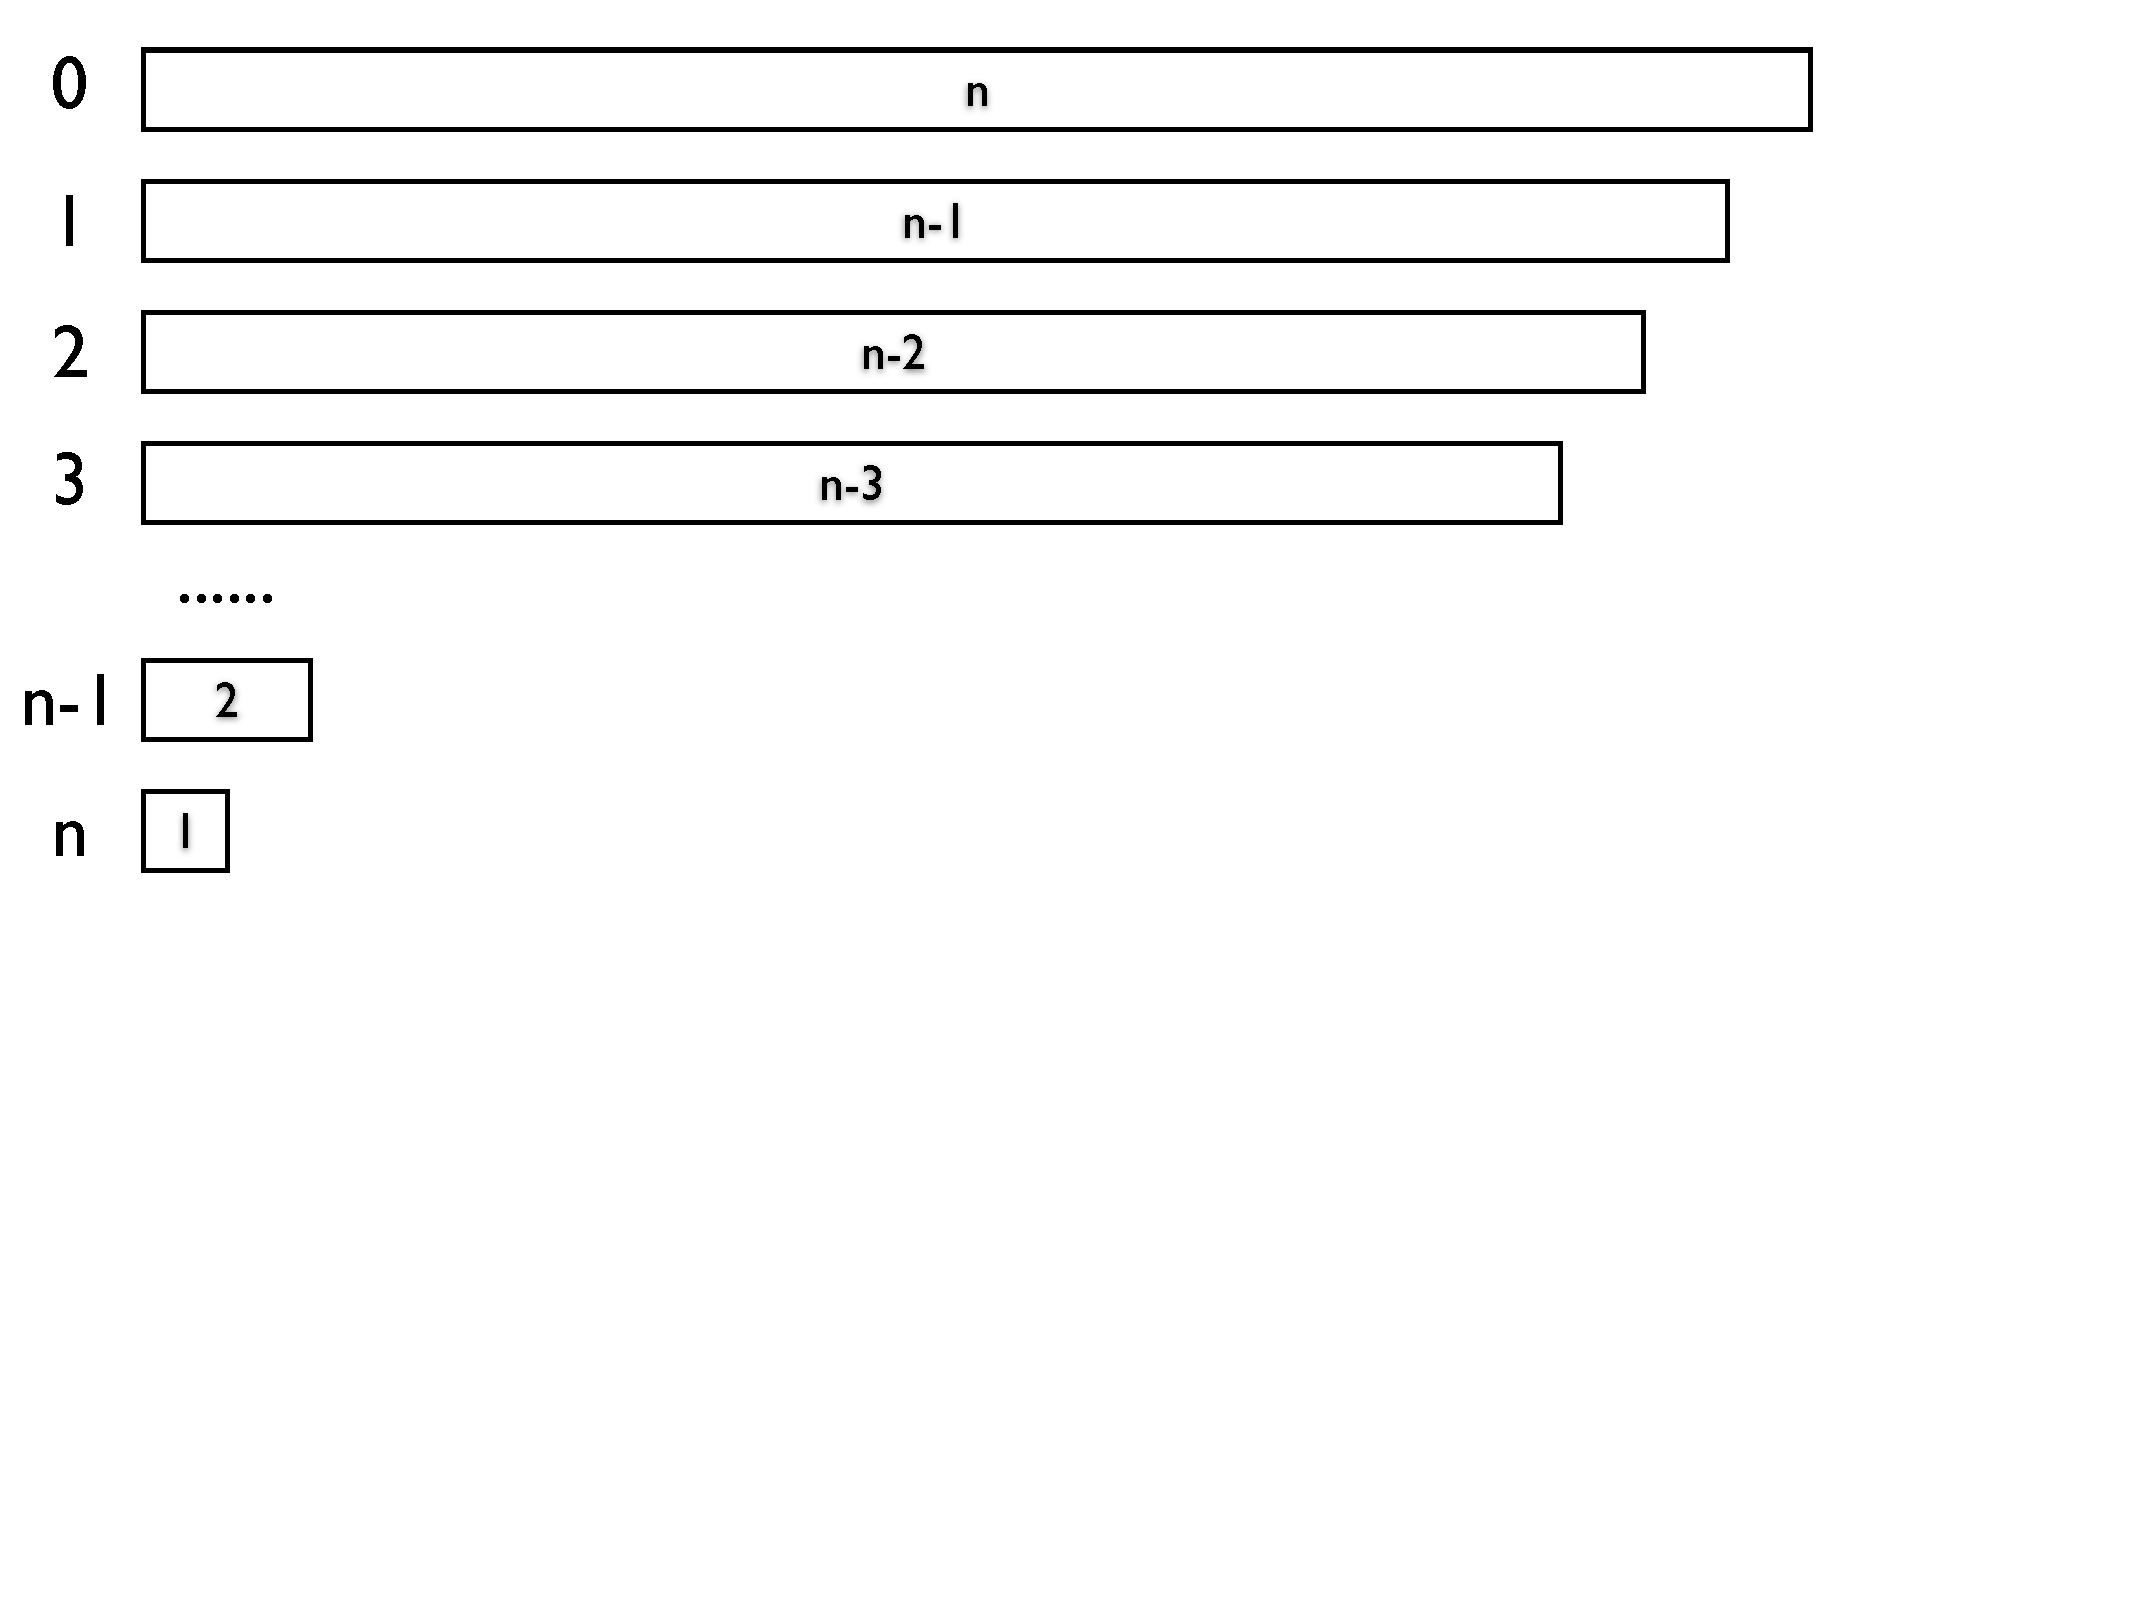
\includegraphics[width=0.7\textwidth]{ennemenouno.pdf}
\end{figure}
\onslide<3|handout:2>
\[
T(n) = \sum_{i=1}^n i = \frac{n (n+1)}{2} = \Theta(n^2)
\]
\end{overprint}

\end{frame}

\begin{frame}{Cosa succede se si sbaglia l'intuizione}

\vspace{-6pt}
\begin{mybox}
\begin{columns}[c]
\begin{column}{0.46\textwidth}
\[
T(n) = \begin{cases}
      T( n-1 )  + n & n > 1 \\
     1 & n \leq 1
  \end{cases}
\]
\end{column}
\begin{column}{0.51\textwidth}
\begingroup\small
\alert{Tentativo sbagliato: $T(n) = O(n)$}\\[2pt]
$\exists c > 0, \exists m \geq 0: T(n) \leq cn, \forall n \geq m$
\endgroup
\end{column}
\end{columns}
\end{mybox}

\BIL
\item \textbf{Ipotesi induttiva}: $\alert{\forall k < n: T(k) \leq c k}$.
\item \textbf{Passo di induzione}: Dimostriamo la disequazione per $T(n)$\\[-6pt]
\begin{flalign*}
  T(n) &=    {T(n-1) + n} \\
       &\leq {c(n-1) + n} && \text{Sostituzione} \\
       &\leq {(c+1)n - c} && \text{Passo algebrico} \\
       &\leq {(c+1)n} && \text{Rimozione elemento negativo} \\
       &\stackrel{?}{\leq} {cn} && \text{Obiettivo} \\
       &\Rightarrow  {c+1 \leq  c} && \text{Impossibile} 
\end{flalign*}
\EIL

\end{frame}

%\subsubsection{Difficoltà matematica}

\begin{frame}{Difficoltà matematica -- Limite superiore}

\vspace{-6pt}
\begin{mybox}
\begin{columns}[c]
\begin{column}{0.64\textwidth}
\[
T(n) = \begin{cases}
      T( \lfloor n/2 \rfloor )  + T( \lceil n/2 \rceil) + 1 & n > 1 \\
     1 & n \leq 1
  \end{cases}
\]
\end{column}
\begin{column}{0.35\textwidth}
\end{column}
\end{columns}
\end{mybox}


\begin{overprint}
\onslide<2|handout:2>
\begin{figure}
	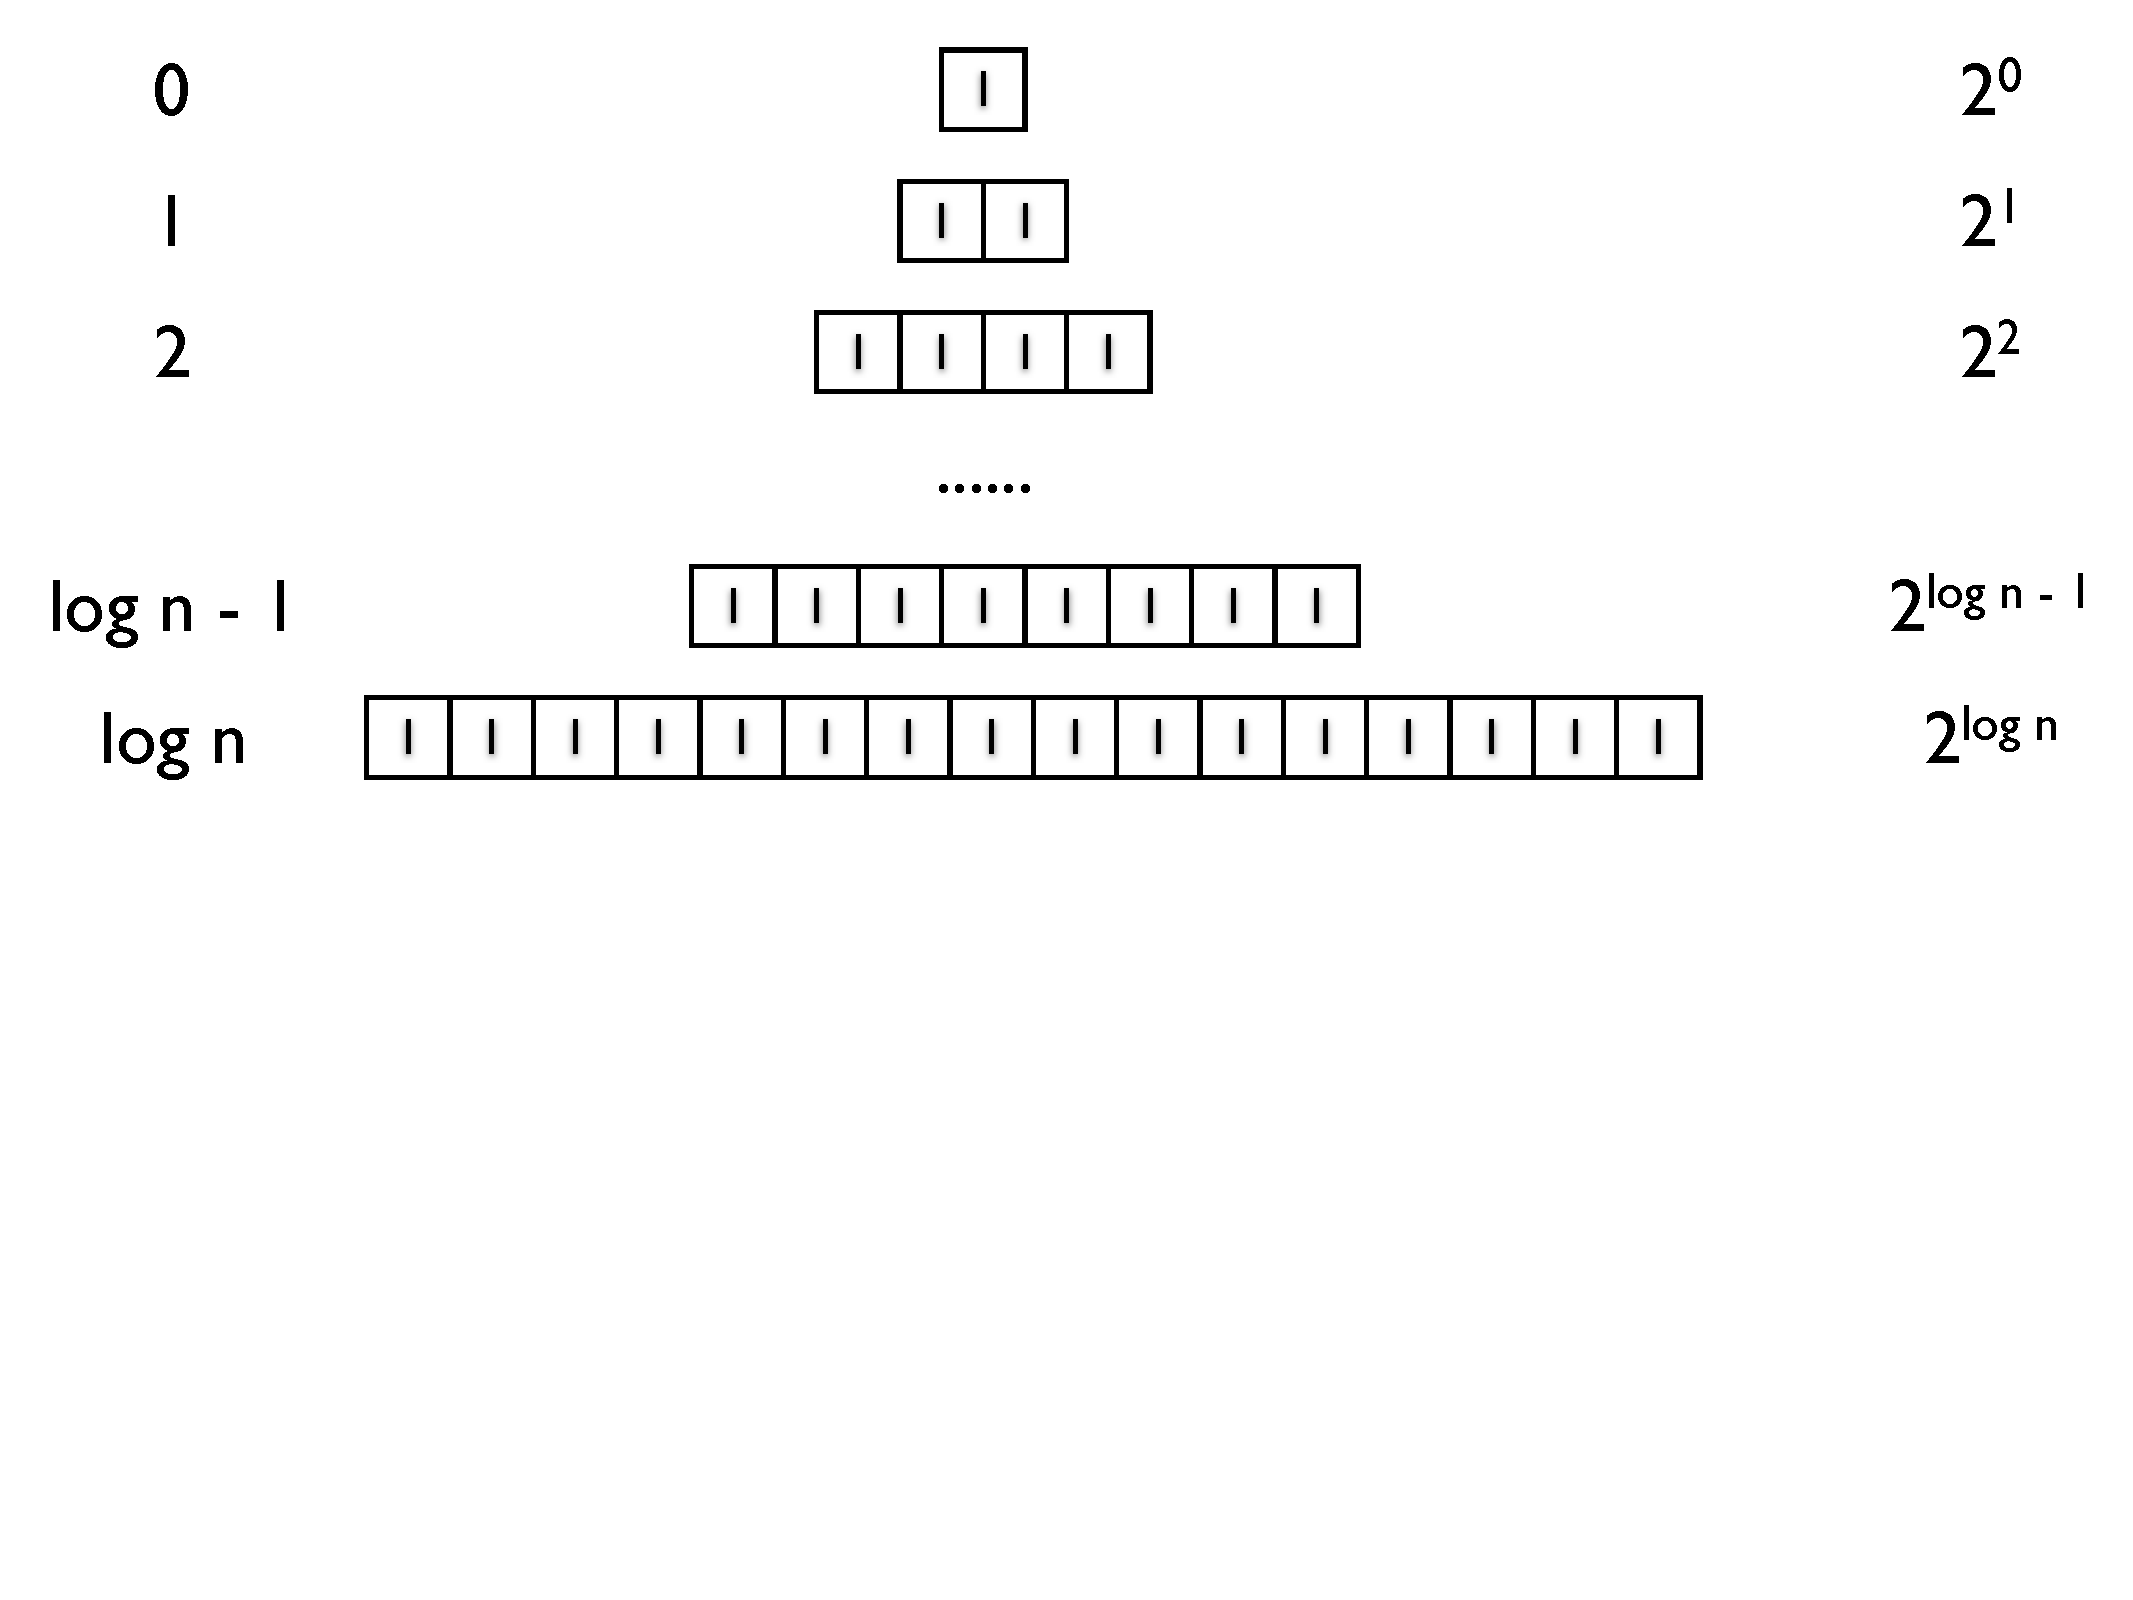
\includegraphics[width=1.0\textwidth]{tree1.pdf}
\end{figure}
\onslide<3|handout:3>
\[
T(n) = \sum_{i=0}^{\log n} 2^i = 1 + 2 + \ldots + n/4 + n/2 + n = O(n)
\]
\end{overprint}

\end{frame}

\begin{frame}{Difficoltà matematica -- Limite superiore}


\vspace{-6pt}
\begin{mybox}
\begin{columns}[c]
\begin{column}{0.64\textwidth}
\[
T(n) = \begin{cases}
      T( \lfloor n/2 \rfloor )  + T( \lceil n/2 \rceil) + 1 & n > 1 \\
     1 & n \leq 1
  \end{cases}
\]
\end{column}
\begin{column}{0.35\textwidth}
\begingroup\small
\alert{Tentativo: $T(n) = O(n)$\\[3pt]}
$\exists c > 0, \exists m \geq 0:$\\
$T(n) \leq cn, \forall n \geq m$
\endgroup
\end{column}
\end{columns}
\end{mybox}

\begin{overprint}
\onslide<1|handout:1>
\BIL
\item \textbf{Ipotesi induttiva}: $\alert{\forall k < n: T(k) \leq c k}$.
\item \textbf{Passo di induzione}: Dimostriamo la disequazione per $T(n)$\\[-6pt]
\begin{flalign*}
  T(n) &=    {T( \lfloor n/2 \rfloor )  + T( \lceil n/2 \rceil) + 1} \\
       &\leq {c \lfloor n/2 \rfloor   + c \lceil n/2 \rceil + 1} && \text{Sostituzione } \\
       &= {cn+1} && \text{Passo algebrico} \\
       &\stackrel{?}{\leq} {cn} && \text{Obiettivo} \\
       &\Rightarrow  {1 \leq  0} && \text{Impossibile} 
\end{flalign*}
\EIL

\onslide<2|handout:2>
\begin{myboxtitle}[Cosa succede?]
\BI
\item Il tentativo è corretto...
\item ma non riusciamo a dimostrarlo per \alert{un termine di ordine inferiore}
\EI	
\[
  cn \alert{+ 1} \leq cn
\]
\end{myboxtitle}	


\onslide<3|handout:3>
\BIL
\item \textbf{Ipotesi induttiva più stretta}: $\alert<1>{\exists b>0, \forall k < n: T(k) \leq c k - b}$.
\item \textbf{Passo di induzione}: Dimostriamo la disequazione per $T(n)$:\\[-6pt]
\begin{flalign*}
  T(n) &=    {T( \lfloor n/2 \rfloor )  + T( \lceil n/2 \rceil) + 1} \\
       &\leq {c \lfloor n/2 \rfloor - b   + c \lceil n/2 \rceil - b + 1} && \text{Sostituzione } \\
       &={cn-2b+1} && \text{Passo algebrico} \\
       &\stackrel{?}{\leq} {cn - b} && \text{Obiettivo} \\
       &\Rightarrow  {-2b+1 \leq -b} && \text{Eliminazione $cn$} \\
       &\Rightarrow  {b \geq 1} && \text{Passo algebrico} 
\end{flalign*}
\EIL
\onslide<4|handout:4>
\BI
\item \textbf{Caso base}: Dimostriamo la disequazione per $T(1)$
	\begin{flalign*}
       T(1) &= 1 \stackrel{?}{\leq} 1 \cdot c - b \Leftrightarrow \forall c \geq b+1 &&
    \end{flalign*}
\EI
\onslide<5|handout:5>
\BIL
	\item Abbiamo provato che $T(n) \leq cn - b \leq cn$
	\BI
		\item \makebox[3.5cm][l]{Nel passo induttivo:} $\forall b \geq 1, \forall c$
		\item \makebox[3.5cm][l]{Nel caso base:} $\forall c \geq b+1$
		\item Una coppia di valori $b,c$ che rispettano queste disequazioni sono $b=1$, $c=2$
	\EI
	\item Questo vale per $n=1$, e per tutti i valori di $n$ seguenti
	\BI
		\item Quindi $m=1$
	\EI
\EIL
\medskip
\begin{mybox}
	Abbiamo quindi provato che $T(n)=O(n)$
\end{mybox}

\end{overprint}

\end{frame}


\begin{frame}[shrink=5]{Difficoltà matematica -- Limite inferiore}

\vspace{-6pt}
\begin{mybox}
\begin{columns}[c]
\begin{column}{0.64\textwidth}
\[
T(n) = \begin{cases}
      T( \lfloor n/2 \rfloor )  + T( \lceil n/2 \rceil) + 1 & n > 1 \\
     1 & n \leq 1
  \end{cases}
\]
\end{column}
\begin{column}{0.35\textwidth}
\begingroup\small
\alert{Tentativo: $T(n) = \Omega(n)$\\[3pt]}
$\exists d > 0, \exists m \geq 0:$\\
$T(n) \geq dn, \forall n \geq m$
\endgroup
\end{column}
\end{columns}
\end{mybox}

\begin{overprint}
\onslide<1>
\BI
\item {\bf Passo di induzione}: Dimostriamo la disequazione per $T(n)$\\[-6pt]
\begin{flalign*}
  T(n) &=    {T( \lfloor n/2 \rfloor )  + T( \lceil n/2 \rceil) + 1} \\
       &\geq {d \lfloor n/2 \rfloor   + d \lceil n/2 \rceil + 1} && \text{Sostituzione } \\
       &= dn+1 \stackrel{?}{\geq} {dn} && \text{Vero per ogni $d$} \\
\end{flalign*}
\vspace{-30pt}
\item {\bf Caso base}: Dimostriamo la disequazione per $T(1)$\\[-6pt]
\begin{flalign*}
  T(n) &= 1 \geq d \cdot 1 \Leftrightarrow d \leq 1 &&
\end{flalign*}
\EI
\end{overprint}

\medskip
\begin{mybox}
	Abbiamo quindi provato che $T(n)=\Omega(n)$
\end{mybox}

\end{frame}



%\subsubsection{Problemi con i casi base}




\begin{frame}{Problemi con i casi base}

\vspace{-6pt}
\begin{mybox}
\begin{columns}[c]
\begin{column}{0.48\textwidth}
\[
T(n) = \begin{cases}
      2T( \lfloor n/2 \rfloor )  + n & n > 1 \\
     1 & n \leq 1
  \end{cases}
\]
\end{column}
\begin{column}{0.51\textwidth}
\end{column}
\end{columns}
\end{mybox}

\begin{overprint}
\onslide<1|handout:1>
\begin{figure}
	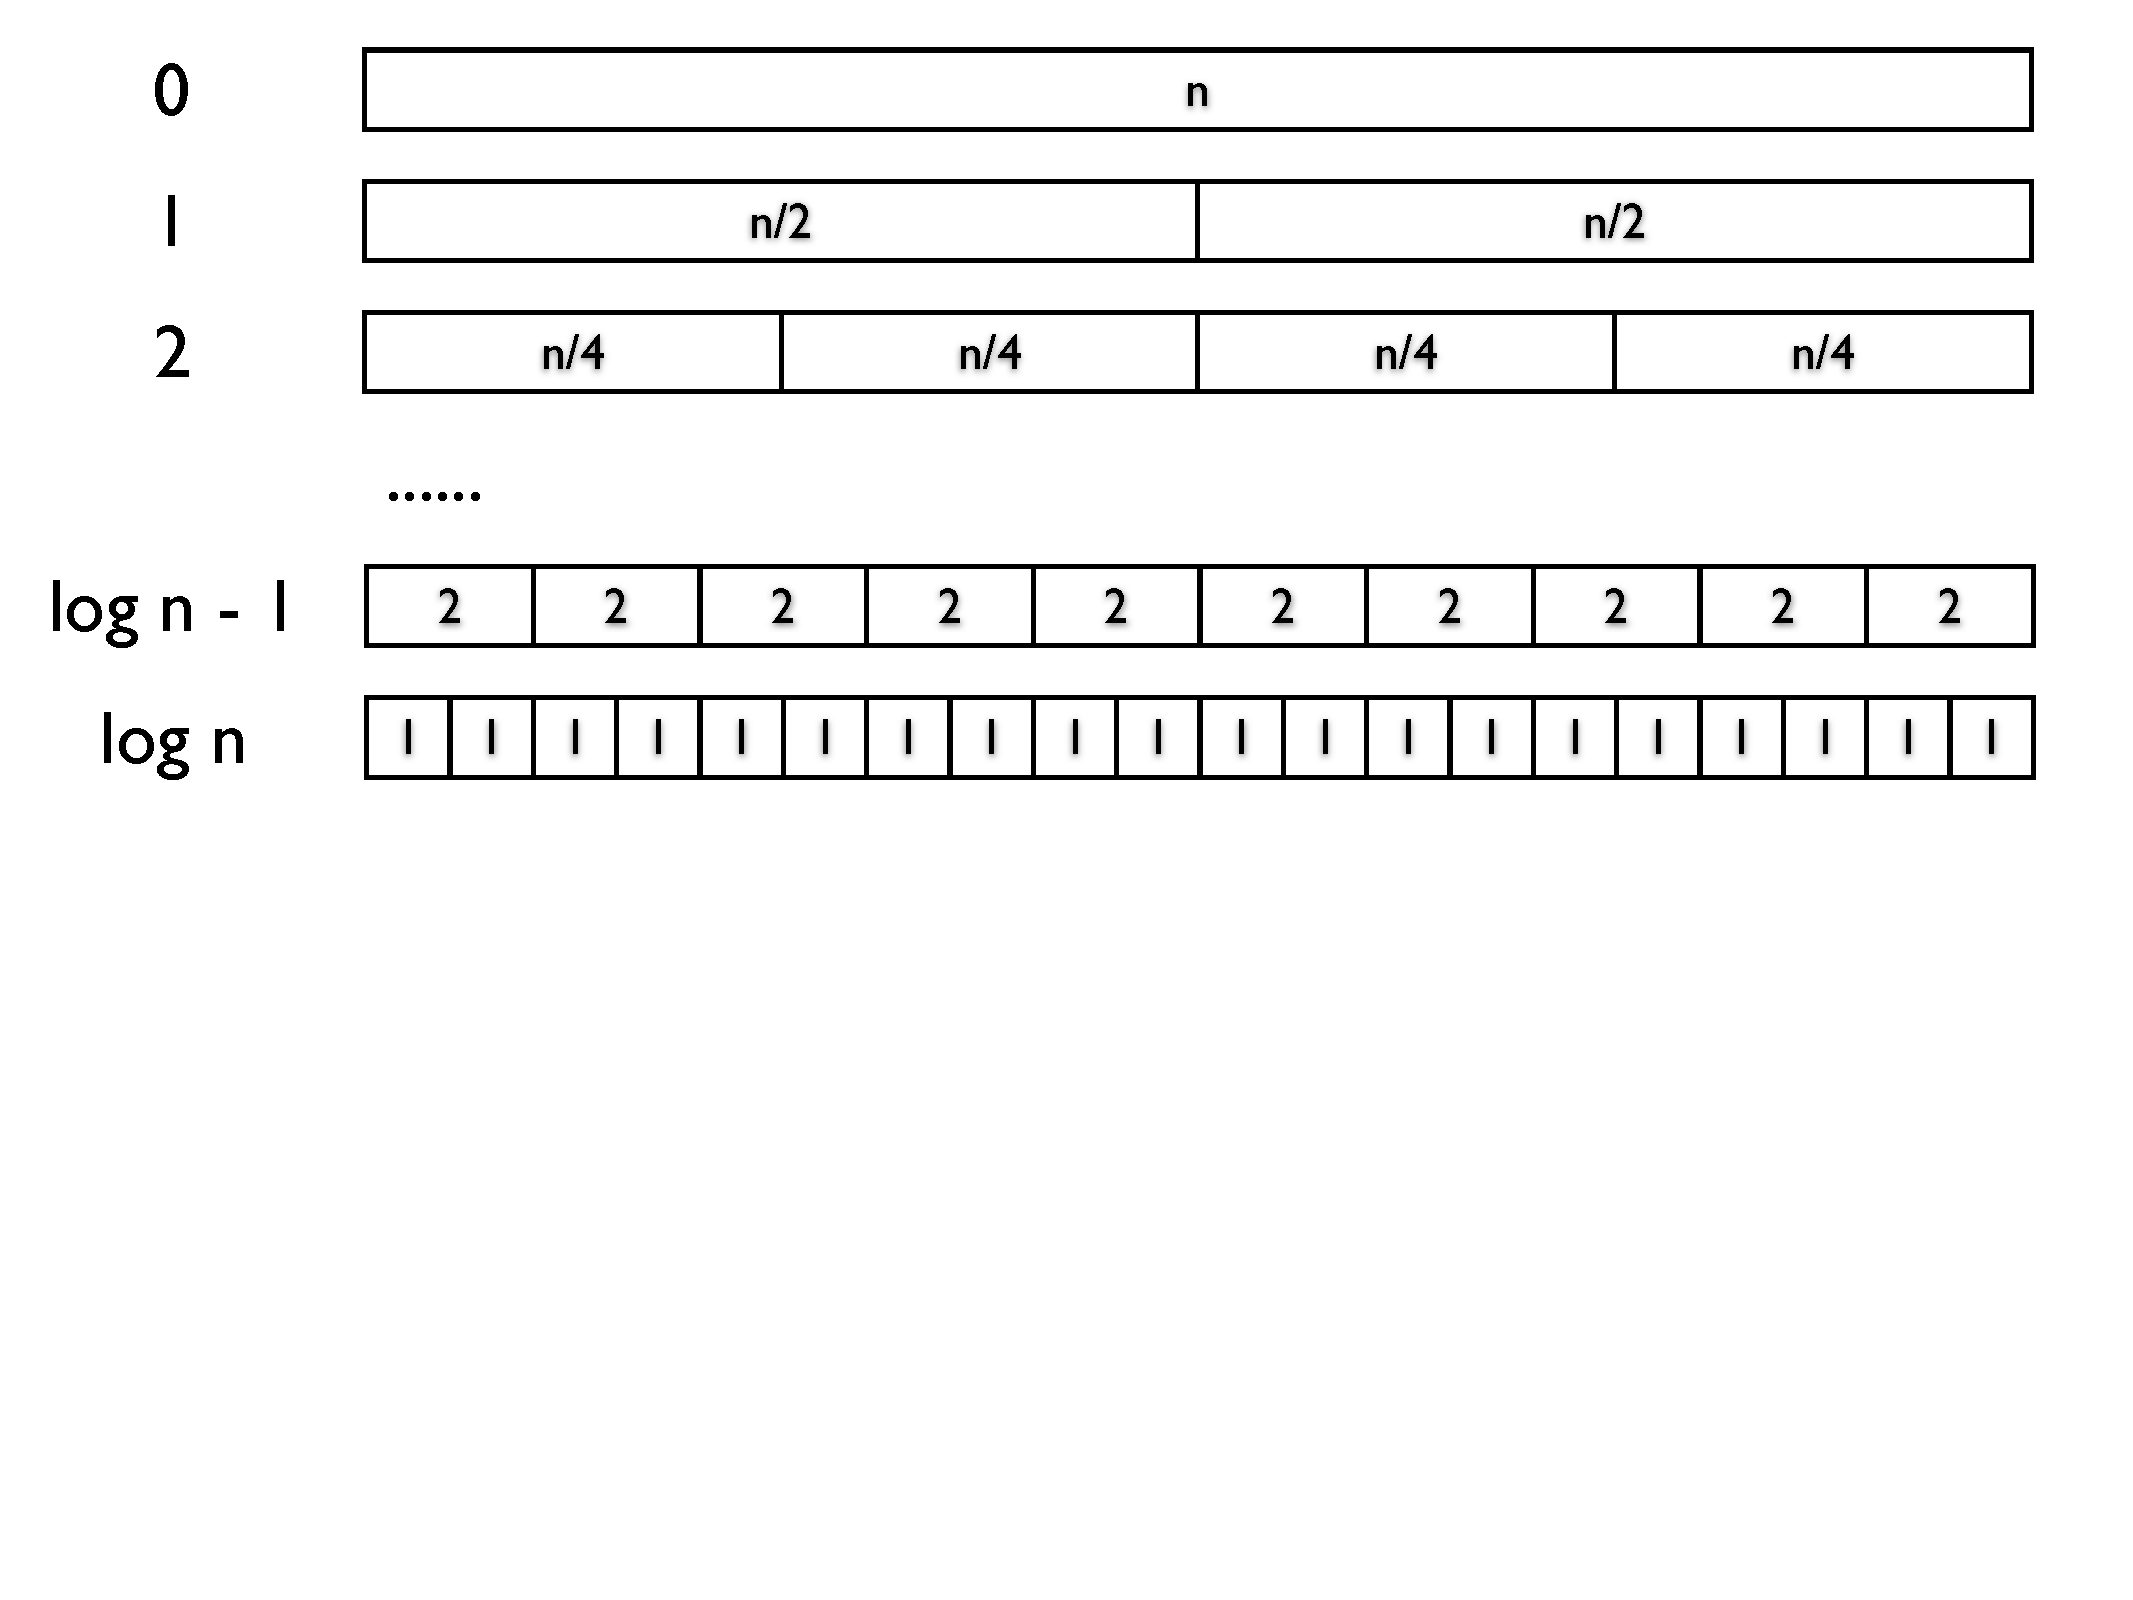
\includegraphics[width=0.9\textwidth]{mergesort.pdf}
\end{figure}
\onslide<2|handout:3>
\[
T(n) = O(n \log n)
\]
\end{overprint}

\end{frame}

\begin{frame}[shrink=5]{Problemi con i casi base}

\vspace{-6pt}
\begin{mybox}
\begin{columns}[c]
\begin{column}{0.48\textwidth}
\[
T(n) = \begin{cases}
      2T( \lfloor n/2 \rfloor )  + n & n > 1 \\
     1 & n \leq 1
  \end{cases}
\]
\end{column}
\begin{column}{0.51\textwidth}
\begingroup\small
\alert{Tentativo: $T(n) = O(n \log n)$}\\
$\exists c > 0, \exists m \geq 0:$ \\
$T(n) \leq cn \log n, \forall n \geq m$
\endgroup
\end{column}
\end{columns}
\end{mybox}

\begin{overprint}
\onslide<1|handout:1>
\BIL
\item \textbf{Ipotesi induttiva}: $\alert{\exists c>0, \forall k < n: T(k) \leq c k \log k}$.
\item \textbf{Passo di induzione}: Dimostriamo la disequazione per $T(n)$:\\[-6pt]
\begin{flalign*}
  T(n) &=    {2 T( \lfloor n/2 \rfloor ) + n} \\
       &\leq {2 c \lfloor n/2 \rfloor \log \lfloor n/2 \rfloor   + n} && \text{Sostituzione } \\
       &\leq {2 cn/2 \log n/2 + n} && \text{Intero inferiore} \\
       &= {cn (\log n - 1) + n}  && \text{Passo algebrico} \\
       &= {cn \log n - cn + n}  && \text{Passo algebrico} \\
       &\stackrel{?}{\leq} {cn \log n} && \text{Obiettivo} 
\end{flalign*}
\EIL
\onslide<2|handout:2>
\BIL
\item \textbf{Ipotesi induttiva}: \alert{$\exists c>0, \forall k < n: T(k) \leq c k \log k$}.
\item \textbf{Passo di induzione}: Dimostriamo la disequazione per $T(n)$:\\[-6pt]
\begin{flalign*}
	T(n) & \leq cn \log n - cn + n \stackrel{?}{\leq} cn \log n && \text{Obiettivo} \\
       &\Rightarrow  {-cn + n \leq 0} && \text{Eliminazione $cn \log n$} \\
       &\Rightarrow  {c \geq 1} && \text{Passo algebrico} \\
\end{flalign*}
\EI

\onslide<3|handout:3>
\BI
\item {\bf Caso base}:  Dimostriamo la disequazione per $T(1)$
	\begin{flalign*}
       T(1) &= 1 \stackrel{?}{\leq} 1 \cdot c \log 1 = 0 \Rightarrow \alert{1 \not\leq 0} &&
    \end{flalign*}
\EI


\onslide<4|handout:4>
\begin{myboxtitle}[Cosa succede?]
  \BIL
    \item \`E falso, ma non è un problema: non a caso si chiama notazione
      asintotica. 
    \item Il valore iniziale di $m$ lo possiamo scegliere noi
  \EIL
\end{myboxtitle}

\onslide<5|handout:5>
\BIL
\item \textbf{Caso base}: Dimostriamo la disequazione per $T(2)$, $T(3)$:\\[-6pt]
	\begin{flalign*}
       T(2) &= {2 T(\lfloor 2/2 \rfloor) + 2 = 4 \leq 1 \cdot c \cdot 2 \log 2 \Leftrightarrow c \geq 2} && \\
       T(3) &= {2 T(\lfloor 3/2 \rfloor) + 3 = 5 \leq 1 \cdot c \cdot 3 \log 3 \Leftrightarrow c \geq \frac{5}{3 \log 3}} &&\\
       T(4) &= {2 T(\lfloor 4/2 \rfloor) + 4 = 2 T(\lfloor 2 \rfloor) + 4} &&
    \end{flalign*}
\item Non è necessario provare la terza disequazione, in quanto viene 
		espressa in base a casi base diversi da $T(1)$ che sono già stati dimostrati
		e quindi possono costituire la base della nostra induzione.
\EI
\onslide<6|handout:6>
\BIL
	\item Abbiamo provato che $T(n) \leq cn \log n$
	\BIL
		\item \makebox[3.5cm][l]{Nel passo induttivo:} $\forall c \geq 1$
		\item \makebox[3.5cm][l]{Nel caso base:} $\forall c \geq 2, c \geq \frac{5}{3 \log 3}$
		\item Visto che sono tutti disequazioni con il segno $\geq$, è sufficiente utilizzare un valore
		  $c \geq \max \{ 1, 2, \frac{5}{3 \log 3} \}$
	\EIL
	\item Questo vale per $n=2, n=3$, e per tutti i valori di $n$ seguenti
	\BIL
		\item Quindi $m=2$
	\EIL
\EIL

\end{overprint}

\end{frame}

\begin{frame}{together now!}
	
\vspace{-6pt}
\begin{mybox}
\begin{columns}[c]
\begin{column}{0.48\textwidth}
\[
T(n) = \begin{cases}
     9 T(\lfloor n/3 \rfloor) + n & n > 1 \\
     1 & n \leq 1 \\
  \end{cases} 
\]
\end{column}
\begin{column}{0.51\textwidth}
\begingroup\small
\alert{Tentativo: $T(n) = O(n^2)$}\\[2pt]
$\exists c > 0, \exists m \geq 0: T(n) \leq cn^2, \forall n \geq m$
\endgroup
\end{column}
\end{columns}
\end{mybox}

\begin{overprint}
\onslide<1|handout:1>
\BIL
\item {\bf Ipotesi induttiva}: $\exists c>0: T(k) \leq ck^2, \forall k < n$
\item {\bf Passo induttivo}: Dimostriamo la disequazione per $T(n)$\\[-6pt]
\begin{flalign*}
T(n) &= 9 T(\lfloor n/3 \rfloor) + n\\
     &\leq 9c(\lfloor n/3 \rfloor)^2 + n && \textrm{Sostituzione}  \\
     &\leq 9c (n^2/9) + n && \textrm{Limite inferiore} \\
     &= cn^2 + n && \textrm{Passo algerbrico}\\
     &\not\leq cn^2 && \textrm{Falso}
\end{flalign*}
\EIL

\onslide<2|handout:2>

\BIL
\item {\bf Ipotesi induttiva}: \alert{$\exists c>0: T(k) \leq c(k^2-k), \forall k < n$}
\item {\bf Passo induttivo}: Dimostriamo la disequazione per $T(n)$\\[-6pt]
\begin{flalign*}
T(n) &= 9 T(\lfloor n/3 \rfloor) + n \\
     &\leq 9c \left(\lfloor n/3 \rfloor^2 - \lfloor n/3 \rfloor\right) + n && \textrm{Sostituzione}\\
     &\leq cn^2 - 3cn + n && \textrm{Limite inferiore}\\
     &\stackrel{?}{\leq} cn^2 -cn  && \textrm{Obiettivo}\\
		 &\Leftrightarrow c \geq \frac{1}{2}
\end{flalign*}
\EIL
	
\onslide<3|handout:3>

\BIL
\item {\bf Ipotesi induttiva}: \alert{$\exists c>0: T(k) \leq c(k^2-k), \forall k < n$}
\item {\bf Passo base}:
\BI
 \item $T(1) = 1 \leq c(1^2-1) = 0$, falso
 \item $T(2) = 9T(0)+ 2 = 11 \leq c(4-2) \Leftrightarrow c \geq 11/2$
 \item $T(3) = 9T(1)+ 3 = 12 \leq c(9-3) \Leftrightarrow c \geq 12/6$
 \item $T(4) = 9T(1)+ 4 = 13 \leq c(16-4) \Leftrightarrow c \geq 13/12$
 \item $T(5) = 9T(1)+ 5 = 14 \leq c(25-5) \Leftrightarrow c \geq 14/20$
 \item $T(6) = 9T(2)+ 6$
\EI
\item Non è necessario andare oltre, perchè $T(6)$ dipende da $T(2)$ che è già 
stato dimostrato
\EIL
	
\onslide<4|handout:4>
	
\BIL
\item Parametri:
\BI
\item $c \geq \max \left\{ \frac{1}{2}, \frac{11}{2}, \frac{12}{6}, \frac{13}{12}, \frac{14}{20} \right\}$	
\item $m=2$
\EI
\item Notare che l'esempio combina le due difficoltà insieme, ma è artificiale:
\BI
\item Se avessimo scelto come ipotesi più stretta \alert{$T(n) \leq cn^2 - bn$}, il
problema sui casi base non si sarebbe posto
\EI
\EIL	

\end{overprint}
	
\end{frame}





%\subsubsection{Conclusioni}

\begin{frame}{Riassumendo}
	
\vspace{-6pt}
\begin{myboxtitle}[Metodo di sostituzione]
\BI
\item Si “\alert{indovina}” una possibile soluzione e si formula un'ipotesi induttiva
\item Si \alert{sostituisce} nella ricorrenza
  le espressioni $T(\cdot)$, utilizzando l'ipotesi induttiva
\item Si \alert{dimostra} che la soluzione è valida anche per il caso base
\EI
\end{myboxtitle}

\begin{myboxtitle}[Attenzione]
\BI
\item Ad ipotizzare soluzioni troppo “strette”
\item Ad alcuni casi particolari che
richiedono alcune astuzie matematiche
\item Attenzione ai casi base: il logaritmo può complicare le cose
\EI
\end{myboxtitle}
\end{frame}

